%%%%%%%%%%%%%%%%%%%%%%%%%%%%%%%%%%%%%%%%%%%%%%%%%%%%%%%%%%%%
% Document settings
\documentclass{ACGSeminar}
\bibliography{references}

%%%%%%%%%%%%%%%%%%%%%%%%%%%%%
% Hyphenations here
%%%%%%%%%%%%%%%%%%%%%%%%%%%%%
\hyphenation{}

%%%%%%%%%%%%%%%%%%%%%%%%%%%%%das erst
% Title, Author, etc.bringt mit sich

\begin{document}

\title{Semi-Lagrangian Approaches for Incompressible Fluid Simulation}

\author{Alexander Enneking}

\maketitle

%%%%%%%%%%%%%%%%%%%%%%%%%%%%%%%%%%%%%%%%%%%%%%%%%%%%%%%%%%%%
% Abstract

\begin{abstract}%

\end{abstract}

\keywords{ }
\tableofcontents

%%%%%%%%%%%%%%%%%%%%%%%%%%%%%%%%%%%%%%%%%%%%%%%%%%%%%%%%%%%%
% Introduction



\section{Introduction}
The goal of the project was to realize a fluid simulation based on \textit{Smoothed Particle Hydrodynamics} (SPH), a method that approximates a continuous volume as a particle cloud, implementing the \textit{Navier Stokes} equations via density estimation.\\
\\
The basic idea behind SPH is to discretize the problem domain - a continuous fluid body - by approximating it using a finite set of particles. Each particle represents a part of the total volume. The goal of SPH is then to model volume preservation under various acting forces using a density estimation as a basis for pressure force exchange between particles as well as friction force computation. Additionally, rigidbodies and boundaries are introduced into the system as sets of locally static particles, with special handling of fluid-rigidbody coupling forces. \\
\\
The project was split into a few iterative steps, given out as bi-weekly assignments.
The first phase was the implementation of a set of kernel functions. These functions are used to the contribution of neighboring particles when computing density, pressure and other values for each individual particle. \\
The kernel functions are chosen such that they satisfy a set of requirements:\\
\begin{enumerate}
\item Normalisation 
\item Symmetry 
\item Delta function property 
\item Non-negativity 
\item Compact support
\end{enumerate}
The first assignment proposed three different functions that satisfy these requirements, as found in [~\cite{Liu}] The cubic spline function, the quintic spline function, and the quadric smooth function.
In our implementation, we mostly use the cubic spline function.\\
\\
These kernel functions are used in all of the subsequent stages, so correctness of implementation was of crucial importance here.\\
\\
The second phase was a first working simulation. It consists of a few steps:\\
\begin{enumerate}
\item Density and pressure estimation
\item Pressure forces and boundary handling
\item Artifical viscosity
\end{enumerate}
The first step lays the computational groundwork for all other calculations as it results in a density estimation for each particle from which a pressure for that particle can be computed.
These values are then used to calculate internal forces for the fluid body in the second step. Additionally, forces between boundary and fluid particles are calculated in order to simulate rigid boundaries to contain the fluid body.
Finally, viscosity is applied by modifying the velocity of each particle.\\
\\
The primitive approach to boundary handling from this phase was then improved in the next phase. \\
Instead of modeling repulsion forces for each boundary particle based on mass and an artificial stiffness parameter, boundary particles are taken into account in the density estimation for fluid particles. The force between a boundary and a fluid particle is then modeled as pressure exchange between the two, weighted by a volume estimation function for the boundary particles to take into account the volume each boundary particle represents and avoid problems with over- or undersampling of boundaries. \\
Additionally, in this phase a position based pressure solver was implemented. In order to achieve the incompressibility property for the fluid, a constraint system is built and solved iteratively. With this approach, each particle is subject to a constraint defined by a function dependent on the particles position, density and the desired rest density.\\
\\
This stage gets rid of artificial stiffness parameters which is supposed to greatly improve stability of the system and reduce problems with inappropriate parameter combinations.  \\
\\
The final assignment consisted of yet another implementation of viscosity, this time to simulate friction forces between fluid particles and boundary particles, implemented as an external force, and a fluid surface reconstruction based on marching cubes. \\
To be able to render an actual fluid instead of a particle cloud, a closed surface must be constructed from the particle cloud. The marching cubes algorithm is a fitting solution to this problem as it is designed to compute hull meshes from a discrete density grid.
The resulting meshes were then to be exported into the .obj file format for each frame of the simulation so they can later be imported and rendered in a 3D graphics program such as the Open Source modeling program Blender.\\
\\

\section{Kernel}

As outlined in the introduction, the first phase of the implementation was implementing three kernel functions - a cubic spline kernel, a quintic spline kernel and a quadric smoothing function kernel. \\
These functions are later to be used to compute a weight for each pair of particles in order to weigh the contribution of a specific particle to another particle's simulation. \\
The input to each function is the distance between two particles and a smoothing length. \\
Kernel functions have to satisfy a set of conditions: \\
\begin{enumerate}
\item Normalisation
\item Symmetry
\item Delta function property
\item Non-negativity
\item Compact support
\end{enumerate}
The normalisation condition requires the integral of the kernel function over the function domain to equal to 1. This guarantees that the sum of all weights will not be larger than one. \\
The symmetry condition guarantees that for each particle pair, the weight function will return the same value no matter the order the particles are input into the function.\\
The delta function property ensures correct behaviour for a vanishing smoothing length.
Non-negativity is obviously required.
Finally, the compact support property makes sure that the kernel function eventually approaches zero for distances greater than the smoothing length.\\
\\
Additionally to the kernel functions, a gradient function had to be implemented for each, as it is required in a few equations later on.
To test the correctness of the gradient functions, we compute the gradient approximately using central differences:\\
\begin{equation} 
\begin{aligned}
\nabla_{x}W(x, h) \approx \nabla^{\epsilon}_{x} W(x, h) = \frac{1}{2\epsilon}\begin{pmatrix}
W(x + \epsilon\mathbf{e}_{x}, h) - W(x - \epsilon\mathbf{e}_{x}, h)\\ 
W(x + \epsilon\mathbf{e}_{y}, h) - W(x - \epsilon\mathbf{e}_{y}, h)\\ 
W(x + \epsilon\mathbf{e}_{z}, h) - W(x - \epsilon\mathbf{e}_{z}, h)\\ 
\end{pmatrix}
\end{aligned}
\end{equation}
\\
We implemented the kernel functions off the equations as given in [\cite{Liu}], deriving the gradient functions for each. However, the first implementation yielded irritating results when testing the gradient for correctness. For the cubic spline kernel, the relative and absolute errors when comparing to the values computed using central differences were far too high. \\
\\
After consulting with another group, we plugged in their implementation for the cubic spline kernel gradient (which should be mathematically equivalent) and noticed the values now being in an acceptable range, so we adapted our implementation to their formula. After this, the curves for the kernel functions looked promising:\\
\\
PICTURE\\
\\
In further development, we mostly used the cubic spline kernel throughout. In hindsight, checking each phase with all kernel functions would have been advisable, as the final implementation shows inconsistent behaviour when switching between kernel functions.\\
\\
A sidenote on the actual implementation, initially we simply used free functions for the different kernel functions and their gradients. Later in development, we switched to a more flexible approach, with each kernel being implemented as a subclass to a generic kernel class. The base kernel class defines an interface to query kernel values as well as gradient values that each kernel type implements. Using object instances also allows to perform a few minor optimizations, like precomputing constant function parameters upon construction. The base class interface allows kernel functions to be swapped out in a single place in the code (even at runtime) instead of having to replace all kernel invocations throughout the codebase.\\
\\

\section{Particle Rendering}
In the second phase of our project we started to implement the actual smoothed particle hydrodynamics method. First we implemented a class which managed the particles and rendered them to the screen. Initially we wanted to use the glviz library for rendering but soon came to the impression that using our own rendering solution would be easier to implement and to maintain and provide more freedom due to a discrepancy between our design philosophy and the design of the library. \\
\\
We started off with a simple shader that projected the particles positions into screen space and displayed them as red dots. We did this by using \verb|GL_POINTS| primitives which does not provide visually pleasing results and lacks perspective projection due to it producing unit-sized screen spaced dots. Yet it was sufficient for visualizing the correctness of our functions. \\
\\
Later on we switched the \verb|GL_POINTS| solution with instanced billboards and achieved spherical results with our blinn-phong based fragment shader. In order to create a sphere from the billboard we provide our fragment shader with the interpolated world-space position of the billboard \(p\) and the interpolated billboard vertex position which, in the billboard-model-space, is the vector from the origin to the billboard position at the current fragment \(\vec{v}\). Du to the billboard being defined from \([-1, -1]\) to \([1, 1]\), we can create a circle by discarding the fragment if \(||\vec{v}|| > 1\). Creating a sphere from the circle can then be done by calculating the vector from the origin to the sphere surface at the current fragment \(\vec{u}\).
\begin{equation} 
\begin{aligned}
||\vec{u}||^2 = 1 = ||\vec{v}||^2 + ||\vec{w}||^2 \Rightarrow ||\vec{w}|| = \sqrt{1 - ||\vec{v}||^2}
\end{aligned}
\end{equation}
With \(\vec{w} = (0,0,||\vec{w}||)\) (due to billboard-model-space).
\begin{equation}
\begin{aligned}
\vec{u} = (\vec{v}.x, \vec{v}.y, \vec{w}.z)
\end{aligned}
\end{equation}
This also yields the surface normal \(\vec{s}_n\) and surface position \(s_p\) and View Matrix \(V\):
\begin{equation}
\begin{aligned}
\vec{s}_n = V^{\text{-}1} \vec{u} \\
s_p = p + V^{\text{-}1} \vec{w} r
\end{aligned}
\end{equation}
These can now be used to calculate the diffuse and specular coefficients \(\Gamma_{diff}, \Gamma_{spec}\) with the light position \(l_{p}\). and the view position \(k_{p}\)
\begin{equation} 
\begin{aligned}
\vec{l}_v &= \frac{l_p - s_p}{||l_p - s_p||}, \quad \vec{k}_v  = \frac{k_p - s_p}{||k_p - s_p||} \\
\Gamma_{diff} &= \vec{s}_n \cdot \vec{l}_v \\
\Gamma_{spec} &= ( \vec{s}_n \cdot \vec{h}) ^ x, \quad \vec{h} = \frac{\vec{l}_n + \vec{k}_n}{||\vec{l}_n + \vec{k}_n||}
\end{aligned}
\end{equation}
With Colors \(C_{ambient}, C_{diff}, C_{spec}\) The Color \(C\) is:
\begin{equation}
\begin{aligned}
C = C_{ambient} + \Gamma_{diff} C_{diff} + \Gamma_{spec} C_{spec}
\end{aligned}
\end{equation}
\begin{figure}[b!]
  \begin{centering}
    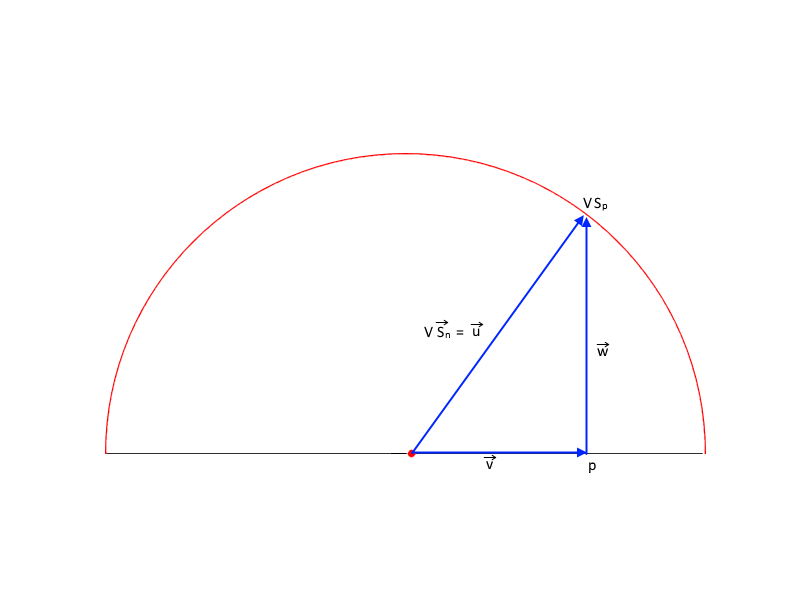
\includegraphics[width=15cm]{figures/particle_shader.png}\par
  \end{centering}
  \caption{The black line is the billboard. The red curve is the sphere surface. The radius is set to one.}
  \label{fig:particle_shader}
\end{figure}

\section{SPH Implementation}
\subsection{Density Estimation}
Performing a density estimation and pressure computation for each particle is the basic building block for the entire simulation.
At the first stage of the implementation, the density estimation takes only fluid particles into account, disregarding boundary particles. The computation is given by the following equation:\\
\begin{equation} 
\begin{aligned}
\rho_i = \sum_j m_j W(||x_i - x_j||,h) 
\end{aligned}
\end{equation}
The density for each particle is equal to the sum of the masses of its neighbours, weighted by the kernel function. Performing the density estimation for each particle and plotting the values results in a graph such as the following:\\
\\
FIGURE: Screenshot density plot\\
\\
The figure shows a plot for particle densities for the initial configuration of a breaking dam scenario.
Densities are distributed mostly uniformly except for particles close to the edges of the fluid body, which are not completely surrounded by other particles.\\
\\
At the second stage of implementation, to improve boundary handling, the density estimation also takes into account boundary particles in the neighborhood of the fluid particle in question. The following equation describes how values are computed now:\\
\\
\begin{equation} 
\begin{aligned}
\rho_{f_{i}} = \sum_{j}m_{f_{j}}W_{ij} + \sum_{k}\Psi_{b_{k}}(\rho_{0})W_{ik}
\end{aligned}
\end{equation}
\\
The equation will be described in more detail later.\\
For both approaches, the pressure value for each particle is computed using the following equation:\\
\begin{equation} 
\begin{aligned}
P_i = \text{max}(B(\rho_i - \rho_0),0)
\end{aligned}
\end{equation}
Here, \(p_0\) describes the rest density for the medium that is being simulated and \(B\) serves as a stiffness coefficient. Similiarly to a spring constraint, pressure increases when the particle configuration is further from a rest configuration. This is a approximation of incompressability, which later is replaced with a position based pressure solver, removing the need for a stiffness coefficient.
During our first implementation, we chose \(B\) far too low (about three or four magnitudes too low), resulting in very odd behaviour at boundary collisions. After consulting [~\cite{Becker}] [\cite{Liu}] [\cite{Akinci}] [\cite{BRIDSON2016}] we were able to correct this mistake.\\
\\
\label{subsec:Pressure Force}
\subsection{Pressure Force}
The first approach towards modeling pressure forces within the fluid given in Assignment 2 was directly computing acceleration values using the following equation:\\
\begin{equation} 
\begin{aligned}
a_{i} = - \sum_{j} m_{j}(\frac{P_{i}}{\rho_{i}^{2}} + \frac{P_{j}}{\rho_{j}^{2}})\nabla_{x_{i}}W(||x_{i} -
 x_{j}||, h)
\end{aligned}
\end{equation}
Here, the kernel gradient function is used to weigh neighbour contributions. 
We implemented this approach without further complications, as well as the semi-implicit Euler method for integration:
\begin{equation} 
\begin{aligned}
v_{i}(t_0 + \Delta t) &= v_i(t_0) + \Delta t  a_i \\
x_i(t_0 + \Delta t) &= x_i(t_0) + \Delta t v_i(t_0 + \Delta t)
\end{aligned}
\end{equation}
With just these equations implemented and without taking gravity into account, we observed the correct behaviour as outlined in the assignment: When distributing particles uniformly in a cube, close enough to each other to exceed the rest density, particles are pushed away from the center of a cube in a radial fashion.\\
This was misleading in a way, as it did cause us to suspect an incorrect implementation of boundary handling when we experienced issues after implementing that, while in truth the pressure computation was off by various magnitudes, as already mentioned. The described scenario simply didn't expose the flaw in our implementation.

\subsection{Boundary Handling: First Pass}

Also in Assignment 2, a first approach to boundary handling was implemented. This approach models boundary particles as force emitters that exceed a force on each fluid particle as given by the following equations:\\
\begin{equation}
\begin{aligned}
f_{ik} &= \frac{m_k}{m_i + m_k} \Gamma(x_k, x_i) \frac{x_i - x_k}{||x_i - x_k||}, \quad q = \frac{1}{h}||x_k - x_i|| \\
\Gamma (x_k, x_i) &= \frac{B_R}{||x_k - x_i||} 
\begin{cases}
\frac{2}{3}  & 0 < q < \frac{2}{3} \\
(2q - \frac{2}{3} q^2)  & \frac{2}{3} < q < 1 \\
\frac{1}{2}(2-q)^2 & 1<q<2 \\
0 & \text{otherwise}
\end{cases}
\end{aligned}
\end{equation}
Broken down, the force exceeded on fluid particle by a boundary particle is given by the relative mass of the boundary particle, weighted by a kernel-like weight function (7) which takes into account the distance between fluid and boundary particle as well as a stiffness coefficient \(B_R\). The force is directed towards the fluid particle.
\(B_R\) was another cause of issues. Same as with the stiffness coefficient \(B\) in the pressure computation, it is not intuitively clear how \(B_R\) should be chosen, and required involved consultation with [PAPERS] to eventually find a good value for it. As with \(B\), the need for this coefficient is removed with the introduction of an improved method. \\
When first implemented, we experienced the problem that boundary forces seemed to act much too strongly, catapulting particles out of the boundaries sometimes, never allowing the body to come to rest.
However, tweaking the parameters that directly control the magnitude of force applied did not improve the behaviour: All values above a certain threshold would lead to no visible change, while values below that threshold would lead to the particles not being reflected at all.
As mentioned before, this was mainly due to our pressure computation being offset by a few magnitudes. After correcting this mistake, boundary forces acted as expected.

\subsection{Boundary Handling: Improved}

As mentioned in the last section, simple boundary handling introduced another stiffness coefficient with a complex, non-obvious value range that is hugely dependent on the scenario. To remove this dependency and also improve stability, Assignment 3 introduced an improved boundary handling algorithm. We already described the adaption of density estimation to take boundary particles into account:\\
\\
\begin{equation} 
\begin{aligned}
\rho_{f_{i}} = \sum_{j}m_{f_{j}}W_{ij} + \sum_{k}\Psi_{b_{k}}(\rho_{0})W_{ik}
\end{aligned}
\end{equation}
\\
This equation takes into account \(\Psi_{b_{k}}\), which is an estimation of the volume each boundary particle represents.
\(\Psi_{b_{k}}\) is computed as follows:\\
\\
\begin{equation} 
\begin{aligned}
\Psi_{\rho_{0}} = \rho_{0}V_{b_{i}}
\end{aligned}
\end{equation}
\\
With 
\begin{equation} 
\begin{aligned}
V_{b_{i}} = \frac{1}{\sum_{k}W_{ik}} 
\end{aligned}
\end{equation}\\
Where \(W_{ij} = W(||x_{i} - x_{x}||, h)\).
This eliminates artifacts due to over- respectively undersampling of boundaries.\\
Forces exceeded on fluid particles by boundary particles can now be written as:\\
\\
\begin{equation} 
\begin{aligned}
F^{p}_{f_{i} \leftarrow b_{j}} = -m_{f_{i}}\Psi_{b_{j}}(\rho_{0})\frac{p_{f_{i}}}{\rho^{2}_{f_{i}}}\nabla W_{ij}
\end{aligned}
\end{equation}\\
\\
Again, this takes into account the volume represented of a boundary particle.\\
It should be noted that there is now no external parameter left, boundary forces are dependent solely on the estimated density and pressure values. The only "arbitary" parameter, the stiffness \(B\) involved in the pressure computation, should vanish in the next step of the implementation.\\

\subsection{Position Based Pressure Solver}

Up to this point, pressure forces were implemented as described in \ref{subsec:Pressure Force}. This has two major drawbacks: The stiffness parameter \(B\), which is non-trivial to find a correct value for, and the lack of incompressiblity. We want to enforce the latter.
For this purpose, a constraint based solution is introduced. Every fluid particle is subject to a constraint function \(C_{i}\).\\
\\
\begin{equation} 
\begin{aligned}
C_{i}(x_{1}, ..., x_{n}) = max (\frac{\rho_{i}}{\rho_{0}} - 1, 0)
\end{aligned}
\end{equation}\\
\\

If we let \(p_i = (x^{T}_1, ..., x^{T}_n)^T\) be a vector that contains all positions of a particle \(i\)'s neighborhood (which includes the particle \(i\), then the goal is to compute a displacement vector \(\Delta p_i\) such that we satisfy \(C_i(p_i + \Delta p_i) = 0\).
To solve this equation, we use Newton iterations. Using the linearized constraint function, for each iteration a projection in gradient direction is computed.
The final displacement is described by \\
\\
\begin{equation}
\begin{aligned}
\Delta x_i = \frac{1}{\rho_0} \sum_j m_j(\lambda_i + \lambda_j) \nabla_{x_j}W(||x_i - x_j||)
\end{aligned}
\end{equation}\\
\\

With \\
\\
\begin{equation}
\begin{aligned}
\lambda_{i} = - \frac{C_{i}}{\sum_{k}||\nabla_{x_{k}}C_{i}||^2 + \epsilon}
\end{aligned}
\end{equation}\\
\\
\begin{equation}
\begin{aligned}
\nabla_{x_{j}} C_{i} = - \frac{m_{j}}{\rho_{0}}\nabla_{x_{j}}W(||x_{i} - x_{j}||, h)
\end{aligned}
\end{equation}\\
\\

The computed displacement is applied to each particles position after integrating external forces like gravity, boundary forces, etc.
After applying the displacement, the velocity for each particle is updated to reflect the distance travelled in the last timestep.
Implementing the given equations did not present a lot of trouble, however, after finishing the implementation, we observed highly incorrect behaviour. While in rest configuration, the simulation would behave as expected, however, once particles were pushed into a tighter configuration that caused their densities to exceed the rest density due to boundary force influence, the system exploded. For each particle, the computed displacement was far too high compared to the expected result.
Inspecting the individual components exposed very high values for \(\lambda\), which was then tracked down to be due to \(\sum_{k}||\nabla_{x_{k}}C_{i}||^2\) evaluating to extremely low values. At the time of this writing, we have not yet found the solution for this problem. The implementation contains the pressure solver, but it exposed the incorrect behaviour described in this paragraph and thus does not deliver any meaningful results.\\

\subsection{Viscosity and Boundary Friction}

In Assignment 2 and Assignment 4 respectively, two types of friction forces were introduced. 
The first type is fluid-internal friction between boundary particles, which is equivalent to fluid viscosity. The approach used here is XSPH viscosity:

\\
\begin{equation}
\begin{aligned}
v^* = v_i + \epsilon \sum_j \frac{m_j}{\rho_j}(v_j - v_i)W(||x_i - x_j||, h)\\
v_i \leftarrow v^*_i
\end{aligned}
\end{equation}\\
\\

Viscosity is applied as a modification of velocity after integration.\\
The second type is friction between boundary particles and fluid particles. In contrast to viscosity, this friction is implemented as an external force.

\\
\begin{equation}
\begin{aligned}
F^v_{f_i \leftarrow b_j} = -m_{f_i}\Psi_{b_j}(\rho_{0_i})\Pi_{ij}\nabla W_{ij}
\end{aligned}
\end{equation}\\
\\

where

\\
\begin{equation}
\begin{aligned}
\Pi_{ij} = -\nu(\frac{min(v_{ij} \cdot x_{ij}, 0)}{||x^2_{ij} + \epsilon h^2||})
\end{aligned}
\end{equation}\\
\\

with

\\
\begin{equation}
\begin{aligned}
\nu = \frac{\alpha h}{2\rho_{f_i}}, x_{ij} = x_i - x_j, v_{ij} = v_i - v_j
\end{aligned}
\end{equation}\\
\\

Here, \(\alpha > 0\) is a viscosity coefficient and \(\epsilon \approx 0.01\) a regularization parameter. 

The implementation for both types of friction was straightforward. In practice, boundary friction would behave well with \(alpha \approx 0.2\) and cause instable behaviour with higher values.
Fluid viscosity would behave as expected, high coefficients effectively result in the simulated body acting more like wax than water. 

\section{Replay System and Multithreading}
A property of the SPH technique is that it is not suited for realtime applications out of the box due to the high computation cost. This makes debugging incorrect behaviour especially difficult. \\
A way to migitate this is parallelizing the implementation. Each stage of the algorithm is trivially parallelizable, as each particle is simulated in isolation. Dependencies only exist on values from previous passes, i.e. pressure forces depend on density and pressure values, but there's no interdependencies during pressure force computation.
This allows to multithread the simulation by partitioning the particles and performing computations for each partition in parallel for each stage.\\
Our implementation automatically divides the set of particles into as many partitions as the executing machine has logical cores (i.e. eight on an Intel i7 with four physical cores and hyperthreading enabled).
Each partition is then updated in separation. Spinlocks are used to ensure that threads stay synchronized across phases, such that no thread starts computation on the next phase until all threads are done with the current phase.\\
Currently the implementation naively launches the worker threads every tick and shuts them down when the tick is over. A better implementation would launch the worker threads only once at startup and send them to sleep when there is no work to be done, but this implementation was a lot simpler to implement and the resulting performance was good enough that the implementation cost of an improved version would have been too high for the benefit.\\
\\
Even with a threaded simulation loop, realtime performance can not be achieved with satisfyingly high particle counts. To allow for debugging and real-time inspection of the simulation nevertheless, we implemented a record+replay system. All the system does is serialize all particle positions into a file for every tick. Existing files can then be read and played back frame by frame. The system also takes care of fixing the replay rate to 60hz, independent of the actual simulation timestep. 
This allows us to record a simulation and play it back in real time, while being able to view it inside the simulation renderer. Having this functionality available was a great help both for debugging purposes and also allows for high fidelity rendition of the simulation at real time in tandem with the surface reconstruction algorithm that was implemented.\\
\\

\section{Surface Reconstruction}
The last of our assignments was to reconstruct the surface of the fluid by using the Marching Cubes algorithm. This algorithm constructs geometry for an implicitly defined surface which we defined as:
\begin{equation} \label{eq:implicit_surface}
\begin{aligned}
S &=\{ x \in \mathbb{R}^3 | \Phi(x) = c \} \\
\Phi(x) &= \sum_j \frac{m_j}{\rho_j} W(||x-x_j||, h)
\end{aligned}
\end{equation}
The first thing we needed to do was to create a mesh. Therefore we created and store vertices between two points such that the resulting rectangular mesh would enclose the boundary box and therefore the fluid assuming that no fluid passes through the boundaries. We construct the vertices such that their distance is \(w\) to each direct neighbour. \\
\\
Next we implemented the method that creates the surface vertices for every frame that we want to render. First we calculate \(\Phi(x)\) for every vertex. We do this by calculating for every particle the box that it is placed in and then adding the corresponding weights to the vertices of the box. Let \(l\) be a vertex of the mesh, such that for all other mesh-vertices \(x\): \(l < x\), then the box that particle \(x_n\) is placed in is \(x_{(i,j,k)},..., x_{(i+1, j+1, k+1)}\) where: 
\begin{equation} \label{eq:implicit_surface}
\begin{aligned}
i = \lfloor \frac{(x_n)_x - l}{w} \rfloor, j &= \lfloor \frac{(x_n)_y - l}{w} \rfloor, k = \lfloor \frac{(x_n)_z - l}{w} \rfloor
\end{aligned}
\end{equation}
Adding \(\frac{m_j}{\rho_j} W(||x-x_j||, h)\) to the vertices weight then yields \(\Phi(x)\). \\
\\
Afterwards we loop through the mesh vertices \((i,j,k)\)  from \((0,0,0)\) to \((i_{max}-1,j_{max}-1,k_{max}-1)\). For Every \((i,j,k)\) we then create a Bitcode. Each bit corresponds to one mesh vertex \(x \in [x_{(i,j,k)}, x_{(i+1,j+1,k+1)}] \) and is \(1\) if \(\Phi(x_{(i,j,k)}) > c\) and \(0\) if \(\Phi(x_{(i,j,k)}) \leq c\). With Eq. ~\ref{eq:implicit_surface} this means that it is \(1\), if the vertex is inside the fluid and \(0\), if the vertex is outside the fluid. The surface vertex positions are then added on the edges depending on the composition of the bits in the corresponding box. Thus we have \(2^8 = 256\) different cases which we represent with an \([256][16]\) array, which maps the bitcode of one box to up to 16 edges where surface vertices have to be added.\\
\\
In order to get the exact positions of the surface-vertices we calculate the linearly interpolated position between the mesh-vertices that correspond to the given edge. Since the two mesh-vertices always only differ in respect of one axis we only have to interpolate along that axis. For example if interpolating the surface-position between \(x_{(i,j,k)}\) and \(x_{(i+1,j,k)}\):
\begin{equation} \label{eq:implicit_surface}
\begin{aligned}
\Gamma_{(i+\frac{1}{2},j,k)} &= \frac{c - \Phi(x_{(i,j,k)})}{\Phi(x_{(i+1,j,k)}) -\Phi(x_{(i,j,k)})} \\
(s_{(i+\frac{1}{2},j,k)})_x &= (x_{(i,j,k)})_x + \Gamma_{(i+\frac{1}{2},j,k)} \\
(s_{(i+\frac{1}{2},j,k)})_{yz} &= (x_{(i,j,k)})_{yz}
\end{aligned} 
\end{equation}
For rendering purposes we also need the normal of every surface vertex:
\begin{equation} \label{eq:implicit_surface}
\begin{aligned}
\vec{n}_{(i+\frac{1}{2},j,k)} = G_{(i,j,k)} + \Gamma * \frac{G_{(i+1,j,k)}-G_{(i,j,k)}}{w}
\\
(G_{(i,j,k)})_x = \Phi_{(i+1,j,k)} - \Phi_{(i-1,j,k)} \\
(G_{(i,j,k)})_y = \Phi_{(i,j+1,k)} - \Phi_{(i,j-1,k)} \\
(G_{(i,j,k)})_z = \Phi_{(i,j,k+1)} - \Phi_{(i,j,k-1)}
\end{aligned} 
\end{equation}
For shading we use Blinn-Phong.

\section{Issues}
\subsection{Neighborhood Search}
We were given an existing implementation of a neighborhood search algorithm. Initially, we used this algorithm wrong, creating a single discretization for all fluid- and boundary particles. This lead to the search being performed on the whole set every tick, which resulted in inacceptable computation times due to the high density and count of boundary particles. We corrected our use such that two separate discretizations are created, one for fluid and one for boundaries, the latter of which does not compute neighbors at all but still takes part in the computation for the fluid particles. This greatly improved performance.\\
We also perform another, completely separate search to speed up volume estimation for boundary particles. As this is performed only once at startup, the performance penalty is acceptable.

\subsection{Smoothing Lengths and Neighboorhod Search Radii}
As mentioned, all kernel functions used in the simulation take into account a smoothing length. The choice of this smoothing length depends on the particle radius - the recommendation we were given is to use a smoothing length equal to four times the particle radius. However, we were a bit unclear on what radius to use for the neighborhood search. 
Intuitively, it makes sense to choose the radius equal to the smoothing length, as neighbors outside of that radius should not contribute to the particle in question at all. However, choosing the radius like that leads to extremely incorrect behaviour at boundaries, causing particles to jump. We have not yet clearified whether this issue is due to a faulty implementation of our kernel functions, or some fundamental misunderstanding in how the different radii relate to one another. We chose a search radius of two times the smoothing length and achieved stable behaviour with this choice.

\subsection{Behaviour of quintic and quadric smoothing function kernels}

When using the quadric smoothing function or the quintic spline kernel instad of the cubic spline kernel, we observe inconsistent behaviour under non-iterative pressure force integration. Using the same start configuration, it seems like the rest density is exceeded with lower distances between particles, leading to the configuration exploding when starting the simulation. The simulation seems stable afterwards and converges towards a behaviour that seems correct, but the initial behaviour seems largely incorrect. We have not found the cause for this at the point of writing.



%%%%%%%%%%%%%%%%%%%%%%%%%%%%%%%%%%%%%%%%%%%%%%%%%%%%%%%%%%%%
% Bibliography

\printbibliography
\cleardoublepage

\end{document}
